\begin{figure}
	\centering
	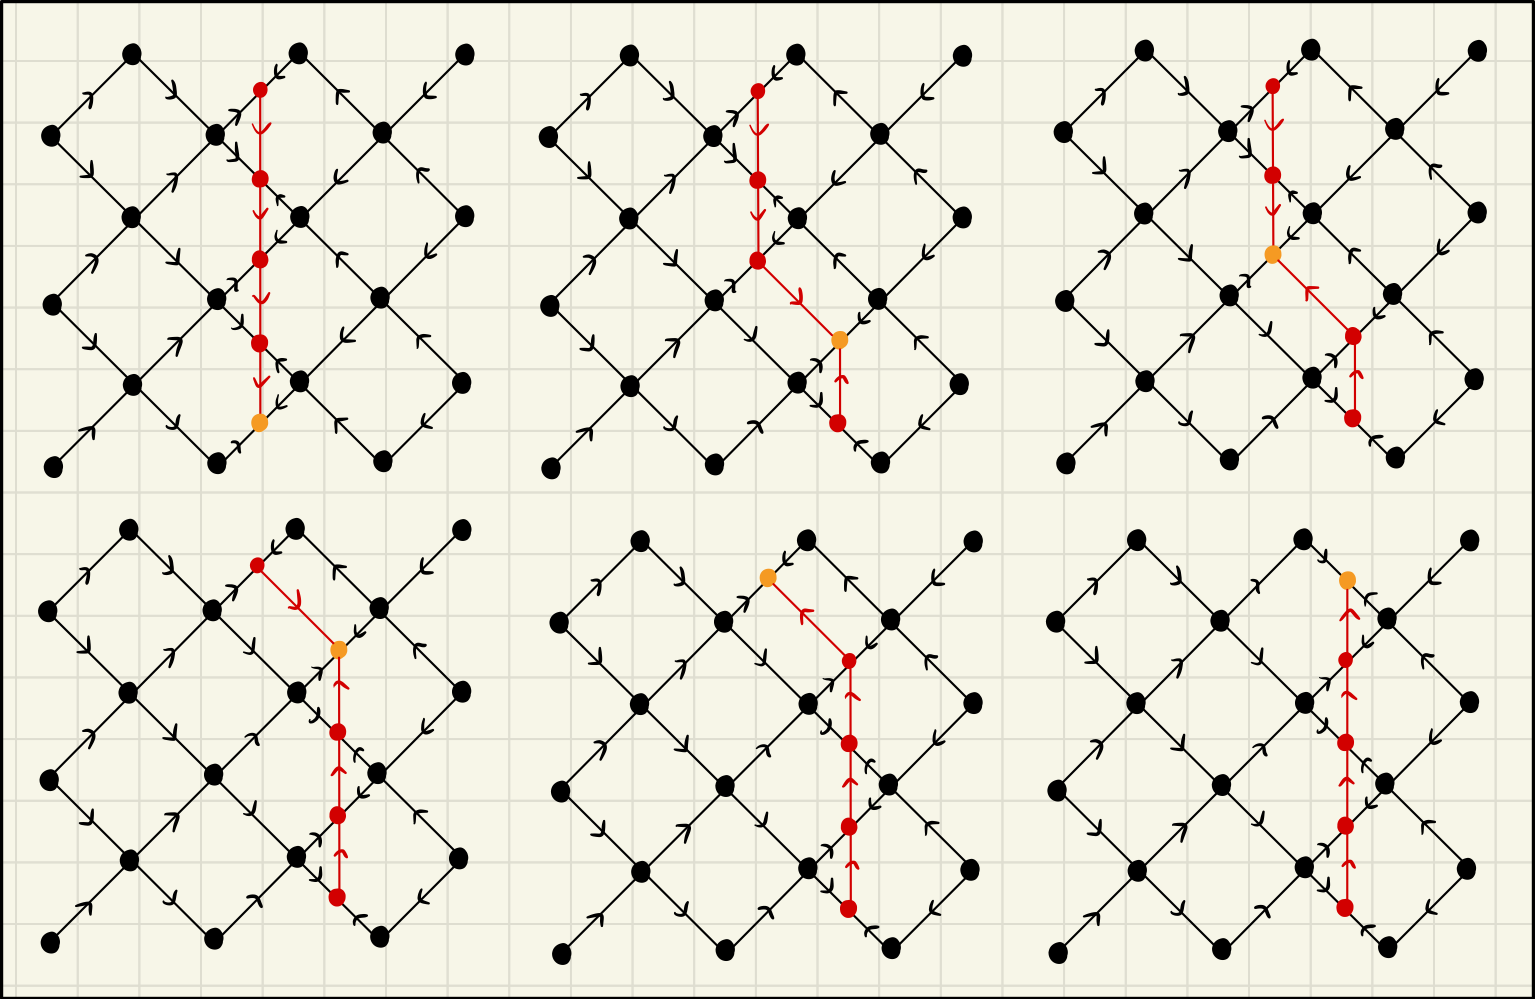
\includegraphics[width=0.9\textwidth]{figures/Tensor_Networks/disoTPS_moving_ortho_surface.jpeg}
	\caption{Two YB-moves are used to shift the orthogonality hypersurface one column to the right. In the last step, the orthogonality center can be moved across the $T$-tensor by contracting the two tensors and performing a QR-decomposition.}
	\label{fig:disoTPS_moving_ortho_surface}
\end{figure}
Most algorithms implemented on disoTPS require an efficient procedure for moving the orthogonality surface, where the error introduced by this procedure should be as small as possible. For isoTPS, the current best procedure is given by the Moses Move, followed by an optional variational optimization. \par
In analogy to the MM we look for a procedure to iteratively shift the orthogonality surface through one column of $T$-tensors as shown in figure \figref{fig:disoTPS_moving_ortho_surface}. A single iteration of this process is shown in figure \figref{fig:disoTPS_YB_move_closeup}. The two tensors $W_1$ and $W_2$, which are part of the orthogonality hypersurface, are "pulled through" the site tensor $T$, resulting in the updated tensors $T^\prime$, $W_1^\prime$ and $W_2^\prime$. To keep the isometric structure of the network, $T^\prime$ and $W_1^\prime$ must be isometries, while $W_2^\prime$ must be a tensor of norm one (the new orthogonality center). Due to the visual similarity to the Yang-Baxter equation we call this procedure the \textit{Yang-Baxter} (YB) move. \par
We denote the state represented by the disoTPS before the YB move by $\left|\Psi\right\rangle = \left|\Psi\left(W_1, W_2, T\right)\right\rangle$ and the state after the YB move by $\left|\Psi^\prime\right\rangle = \left|\Psi^\prime\left(W_1^\prime, W_2^\prime, T^\prime\right)\right\rangle$. One can think of the YB move as a constrained optimization problem
\begin{equation}
	\label{eq:disoTPS_YB_move_standard}
	\left(T^\prime, W_1^\prime, W_2^\prime\right) = \underset{T^\prime,W_1^\prime,W_2^\prime}{\text{min}}\left\lVert \left|\Psi\right\rangle - \left|\Psi^\prime\right\rangle\right\rVert,
\end{equation}
\begin{equation}
	\label{eq:disoTPS_YB_move_constraints}
	T^{\prime\dagger}T^\prime = \id, \quad W_1^{\prime\dagger}W_1^\prime = \id, \quad \left\lVert W_2^\prime \right\rVert = 1.
\end{equation} \par
\begin{figure}
	\centering
	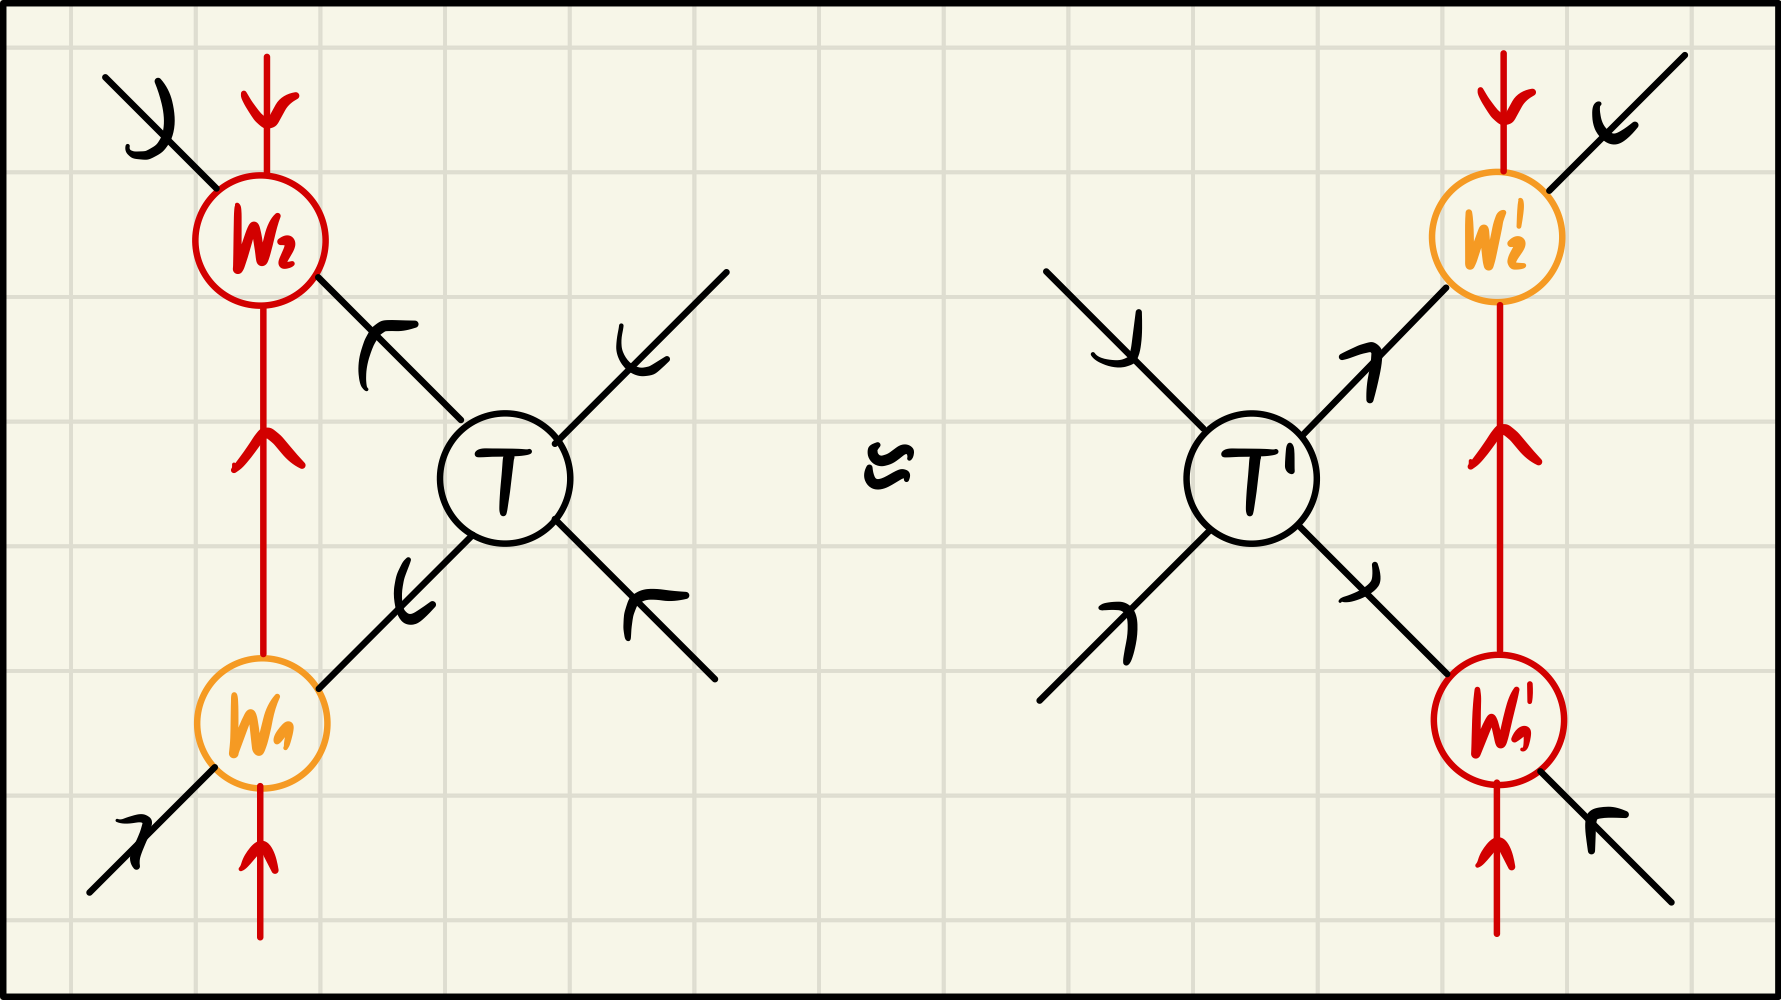
\includegraphics[width=0.9\textwidth]{figures/Tensor_Networks/YB_move_closeup.jpeg}
	\caption{The Yang-Baxter (YB) move is the procedure of "pulling" two auxillary tensors $W_1$ and $W_2$ through a site tensor $T$.}
	\label{fig:disoTPS_YB_move_closeup}
\end{figure}
In the following, we present two explicit algorithms for performing the YB move. The first algorithm is an iterative optimization using local updates respecting the constraints. The second algorithm is a tripartite decomposition with disentangling similar to the tripartite decomposition used in the MM. In section \ref{} we will compare the two algorithms.

\subsection{Iterative optimization with local updates}
\label{sec:YB_move_iterative_local_optimization}
We can rewrite the error of the YB move as
\begin{equation}
	\begin{split}
		\left\lVert \left|\Psi\right\rangle - \left|\Psi^\prime\right\rangle \right\rVert_\text{F} =& \sqrt{\left\langle\Psi\middle|\Psi\right\rangle + \left\langle\Psi^\prime\middle|\Psi^\prime\right\rangle - 2\Re\left\langle\Psi\middle|\Psi^\prime\right\rangle} \\
		=& \sqrt{2 - 2\Re\left\langle\Psi\middle|\Psi^\prime\right\rangle},
	\end{split}
\end{equation}
where in the second step we used the fact that the wave function is normalized to one, $\left\langle\Psi\middle|\Psi\right\rangle = \left\langle\Psi^\prime\middle|\Psi^\prime\right\rangle = 1$. It follows that the optimization problem of minimizing the error becomes the problem of maximizing the overlap
\begin{equation}
	\label{eq:disoTPS_YB_move_alternative_formulation}
	\left(T^\prime, W_1^\prime, W_2^\prime\right) = \underset{T^\prime,W_1^\prime,W_2^\prime}{\text{argmax}}\Re\left\langle\Psi\middle|\Psi^\prime\right\rangle
\end{equation}
under the constraints \eqref{eq:disoTPS_YB_move_constraints}. Because the only tensors that are changed by the YB move are $W_1$, $W_2$ and $T$ and the three tensors make up a subregion of the full network with only incoming arrows, we can use the isometry condition and the computation of the overlap reduces to a contraction of only six tensors as shown in figure \figref{fig:YB_move_iterate_polar_overlap}. We proceed by keeping all tensors fixed except one of the three tensors $T^\prime$, $W_1^\prime$ or $W_2^\prime$ and optimizing the overlap. We can then iterate over the three tensors to converge to a solution. \par
We first show how the tensor $W_2^\prime$ can be optimized. We treat all tensors except $W_2^\prime$ as constant and contract them into an environment $E$ as shown in figure \figref{fig:YB_move_iterate_polar_optimize_W2}. One can then write the optimization problem as
\begin{equation}
	\label{eq:disoTPS_YB_move_optimization_problem_W_2_prime}
	W_2^\prime = \underset{\lVert W_1^\prime \rVert = 1}{\text{argmax}} \Re\left\langle\Psi\middle|\Psi^\prime\right\rangle = \underset{\lVert W_1^\prime \rVert = 1}{\text{argmax}} \Re\left\langle W_2^\prime, E \right\rangle_\text{F},
\end{equation}
with the Frobenius inner product $\left\langle \cdot, \cdot \right\rangle_\text{F}$ \eqref{eq:frobenius_inner_product}. The Frobenius inner product satisfies the Cauchy-Schwarz inequality and we obtain
\begin{equation}
	\left|\Re\left\langle W_2^\prime, E \right\rangle_\text{F}\right| \le \lVert W_2^\prime\rVert\lVert E\rVert = \lVert E\rVert.
\end{equation}
If we set $W = E/\lVert E\rVert$ we obtain
\begin{equation}
	\Re\left\langle W_2^\prime, E \right\rangle_\text{F} = \frac{\Re\left\langle E^\prime, E \right\rangle_\text{F}}{\lVert E\rVert} = \lVert E\rVert
\end{equation}
and the maximum is reached. Thus, the closed form solution to \eqref{eq:disoTPS_YB_move_optimization_problem_W_2_prime} is $W_2^\prime = E/\lVert E\rVert$. \par
Next, we optimize the tensor $W_1^\prime$. Again, we keep all other tensors fixed and contract them into the environment $E$ as shown in figure \figref{fig:YB_move_iterate_polar_optimize_W1}. We now reshape $E$ into a matrix, grouping together all legs that connect to legs of $W_1^\prime$ decorated with incoming/outgoing arrows respectively (see figure \figref{fig:YB_move_iterate_polar_optimize_W1}). For the bond dimensions specified in figure \figref{fig:YB_move_iterate_polar_overlap}, $E$ is a complex $\chi D^2 \times \chi$ matrix. The optimization problem can then be written as
\begin{equation}
	\label{eq:disoTPS_YB_move_optimization_problem_W_1_prime}
	W_1^\prime = \underset{W_1^{\prime\dagger}W_1^\prime = \id}{\text{argmax}}\Re\left\langle\Psi\middle|\Psi^\prime\right\rangle = \underset{W_1^{\prime\dagger}W_1^\prime = \id}{\text{argmax}} \Re\left\langle W_1^\prime, E \right\rangle_\text{F} = \underset{W_1^{\prime\dagger}W_1^\prime = \id}{\text{argmax}} \Re\Tr\left(W_1^{\prime\dagger}E\right),
\end{equation}
where $W_1^\prime$ has the same dimensions as $E$. This is known as the \textit{orthogonal procrustes problem} and permits a closed-form solution. \todo{cite something for the procrustes problem?} Taking the SVD of $E$ yields $E = USV^\dagger$. Note that, because of the shape of $E$, $V$ is a $\chi\times\chi$ unitary. Inserting the SVD into the trace yields
\begin{equation}
	\begin{split}
	\Re\Tr\left(W_1^{\prime\dagger}E\right) &= \Re\Tr\left(E W_1^{\prime\dagger}\right) = \Re\Tr\left(USV^\dagger W_1^{\prime\dagger}\right)\\
	&= \Re\Tr\left[\left(U\sqrt{S}\right)\left(\sqrt{S}V^\dagger W_1^{\prime\dagger}\right)\right] = \Re\left\langle\sqrt{S}U^\dagger,\sqrt{S}V^\dagger T^{\prime\dagger}\right\rangle_\text{F}.
	\end{split}
\end{equation}
We again use the Cauchy-Schwarz inequality to obtain an upper bound
\begin{equation}
	\begin{split}
		\left|\Re\Tr\left(W_1^{\prime\dagger}E\right)\right| &= \left|\Re\left\langle\sqrt{S}U^\dagger,\sqrt{S}V^\dagger T^{\prime\dagger}\right\rangle_\text{F}\right| \le \left\lVert\sqrt{S}U^\dagger\right\rVert_\text{F} \left\lVert\sqrt{S}V^\dagger T^{\prime\dagger}\right\rVert_\text{F}\\
		&= \sqrt{\Tr\left(USU^\dagger\right)\Tr\left(T^\prime VSV^\dagger T^{\prime\dagger}\right)} = \Tr\left(S\right),		
	\end{split}
\end{equation}
where in the last step we used $U^\dagger U = \id$, $V^\dagger V = \id$, $W_1^{\prime\dagger}W_1^\prime = \id$ and the cyclic property of the trace. The upper bound can be reached by setting $W_1^\prime = UV^\dagger$:
\begin{equation}
	\Re\Tr\left(W_1^{\prime\dagger}E\right) = \Re\Tr\left(VU^\dagger USV^\dagger\right) = \Tr\left(S\right).
\end{equation}\par
Lastly we show how the tensor $T^\prime$ can be optimized. Similar to the optimization of $W_1^\prime$, we obtain an orthogonal Procrustes problem after contracting the environment $E$ and performing an SVD $E = USV^\dagger$ as shown in figure \figref{fig:YB_move_iterate_polar_optimize_T}. Again, the closed form solution is given by $T^\prime = UV^\dagger$. To summarize, the complete procedure is given in algorithm \ref{alg:YB_iterate_polar}. In practice, one can compute the remaining error after each iteration and terminate the while loop if the decrease in error is smaller than a given threshold or if a given maximum number of iterations is reached.
\begin{algorithm}
	\caption{iterative YB optimization with local updates}
	\label{alg:YB_iterate_polar}
	\begin{algorithmic}
		\Require tensors $T, W_1, W_2, T^\prime, W_1^\prime, W_2^\prime$ as in figure \figref{fig:YB_move_iterate_polar_overlap}
		\Ensure Optimized tensors $T^\prime, W_1^\prime, W_2^\prime$ minimizing the truncation error \eqref{eq:disoTPS_YB_move_standard}
		\While{not converged}
		\State $E \gets \text{contract}\left(T, W_1, W_2, W_1^\prime, W_2^\prime\right)$
		\State $U, S, V^\dagger \gets \text{SVD}\left(E\right)$
		\State $T^\prime \gets UV^\dagger$
		\State $E \gets \text{contract}\left(T, W_1, W_2, T^\prime, W_2^\prime\right)$
		\State $U, S, V^\dagger \gets \text{SVD}\left(E\right)$
		\State $W_1^\prime \gets UV^\dagger$
		
		\State $E \gets \text{contract}\left(T, W_1, W_2, T^\prime, W_1^\prime\right)$
		\State $W_2^\prime \gets E/\lVert E\rVert$
		\EndWhile
	\end{algorithmic}
\end{algorithm}
\todo{Discuss complexity!}
\begin{figure}
	\centering
	\subcaptionbox{\label{fig:YB_move_iterate_polar_overlap}}
	{%
		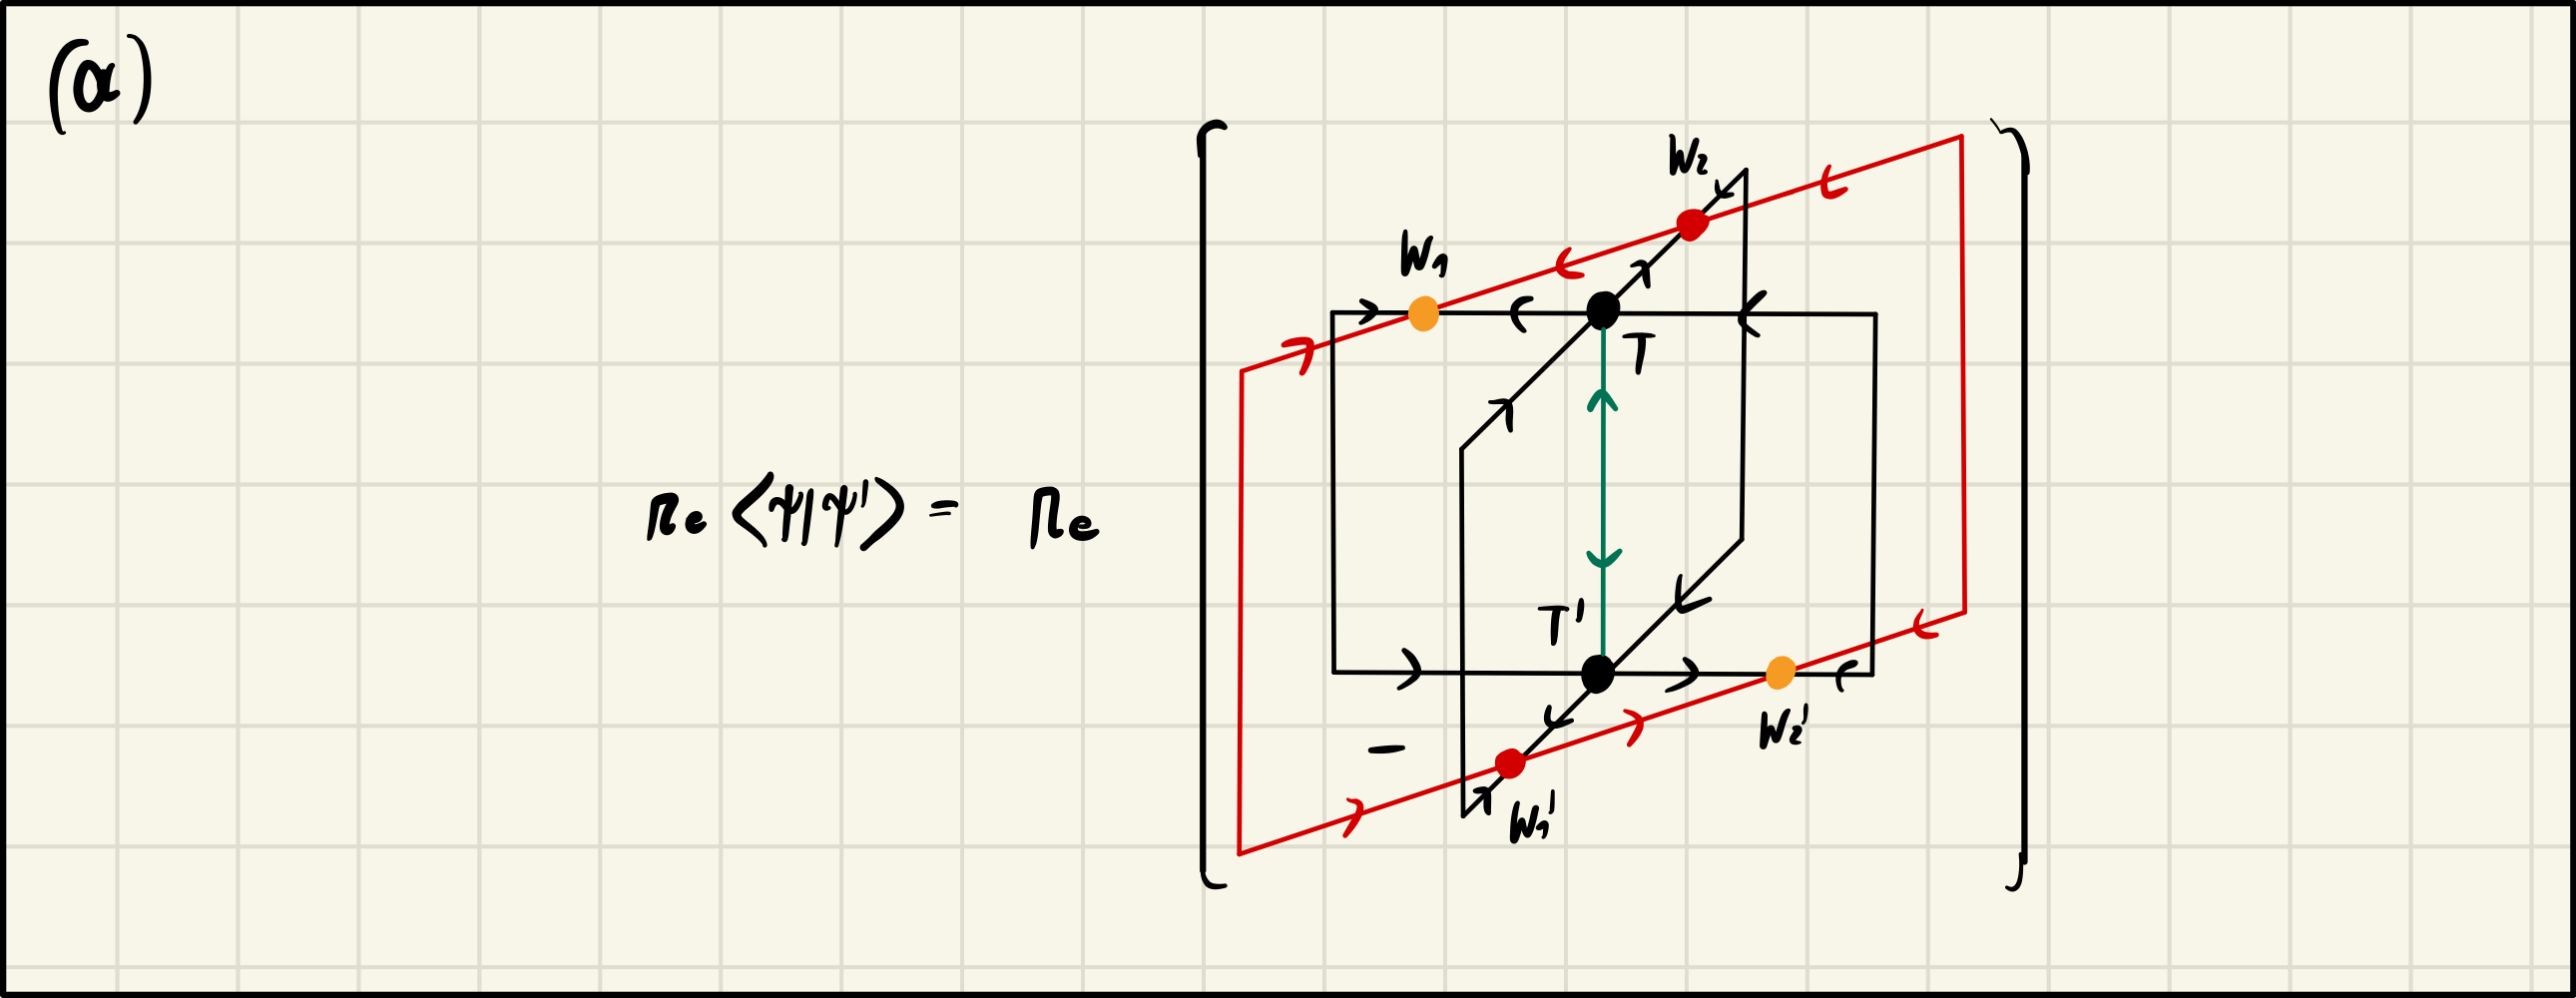
\includegraphics[width=0.7\textwidth]{figures/disoTPS/YB_move_iterate_polar_a.jpeg}
	}
	\subcaptionbox{\label{fig:YB_move_iterate_polar_optimize_W2}}
	{%
		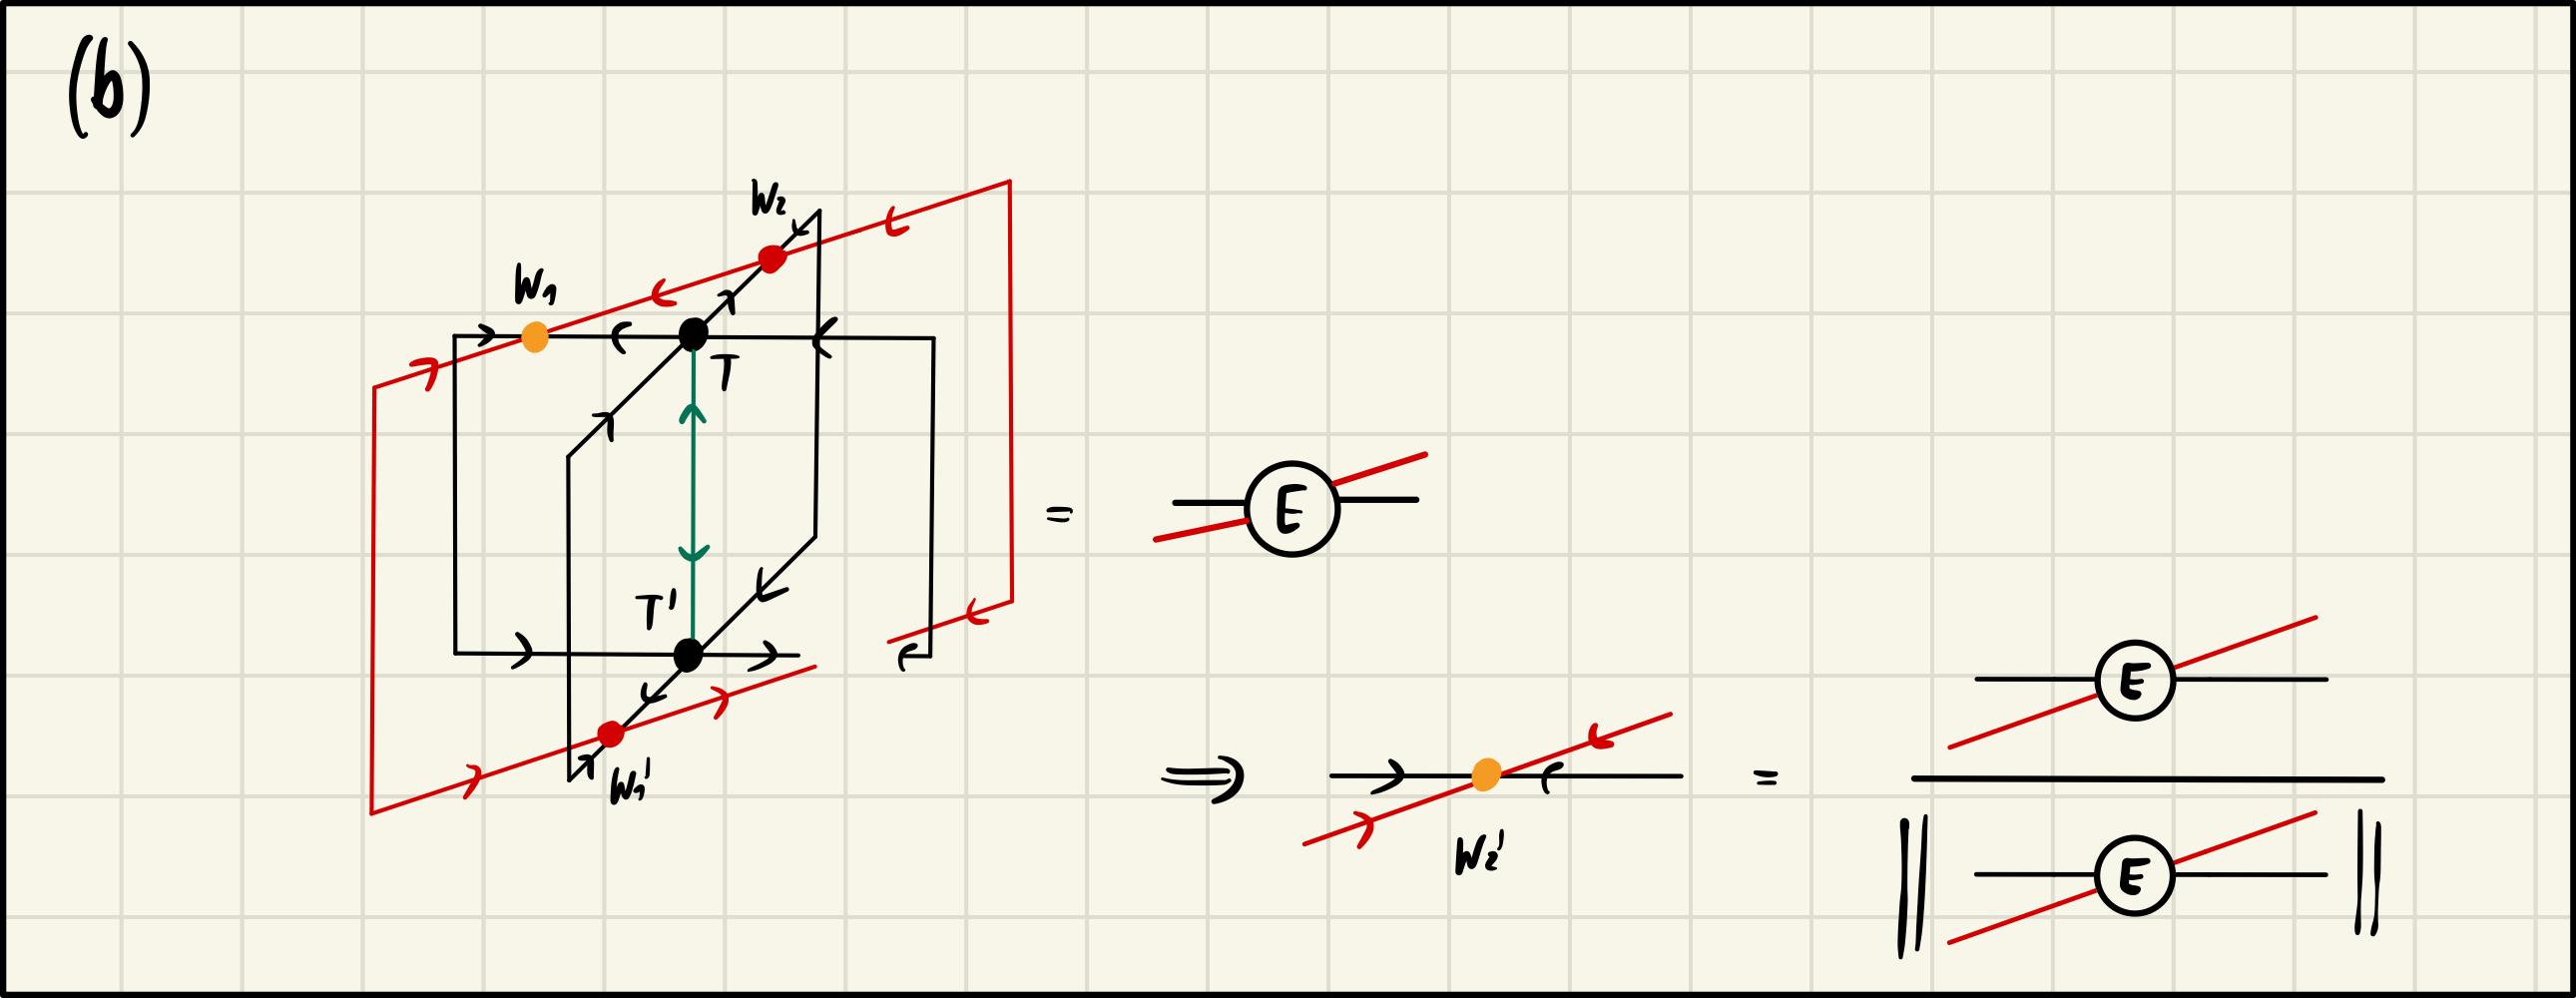
\includegraphics[width=0.7\textwidth]{figures/disoTPS/YB_move_iterate_polar_b.jpeg}
	}
	\subcaptionbox{\label{fig:YB_move_iterate_polar_optimize_W1}}
	{%
		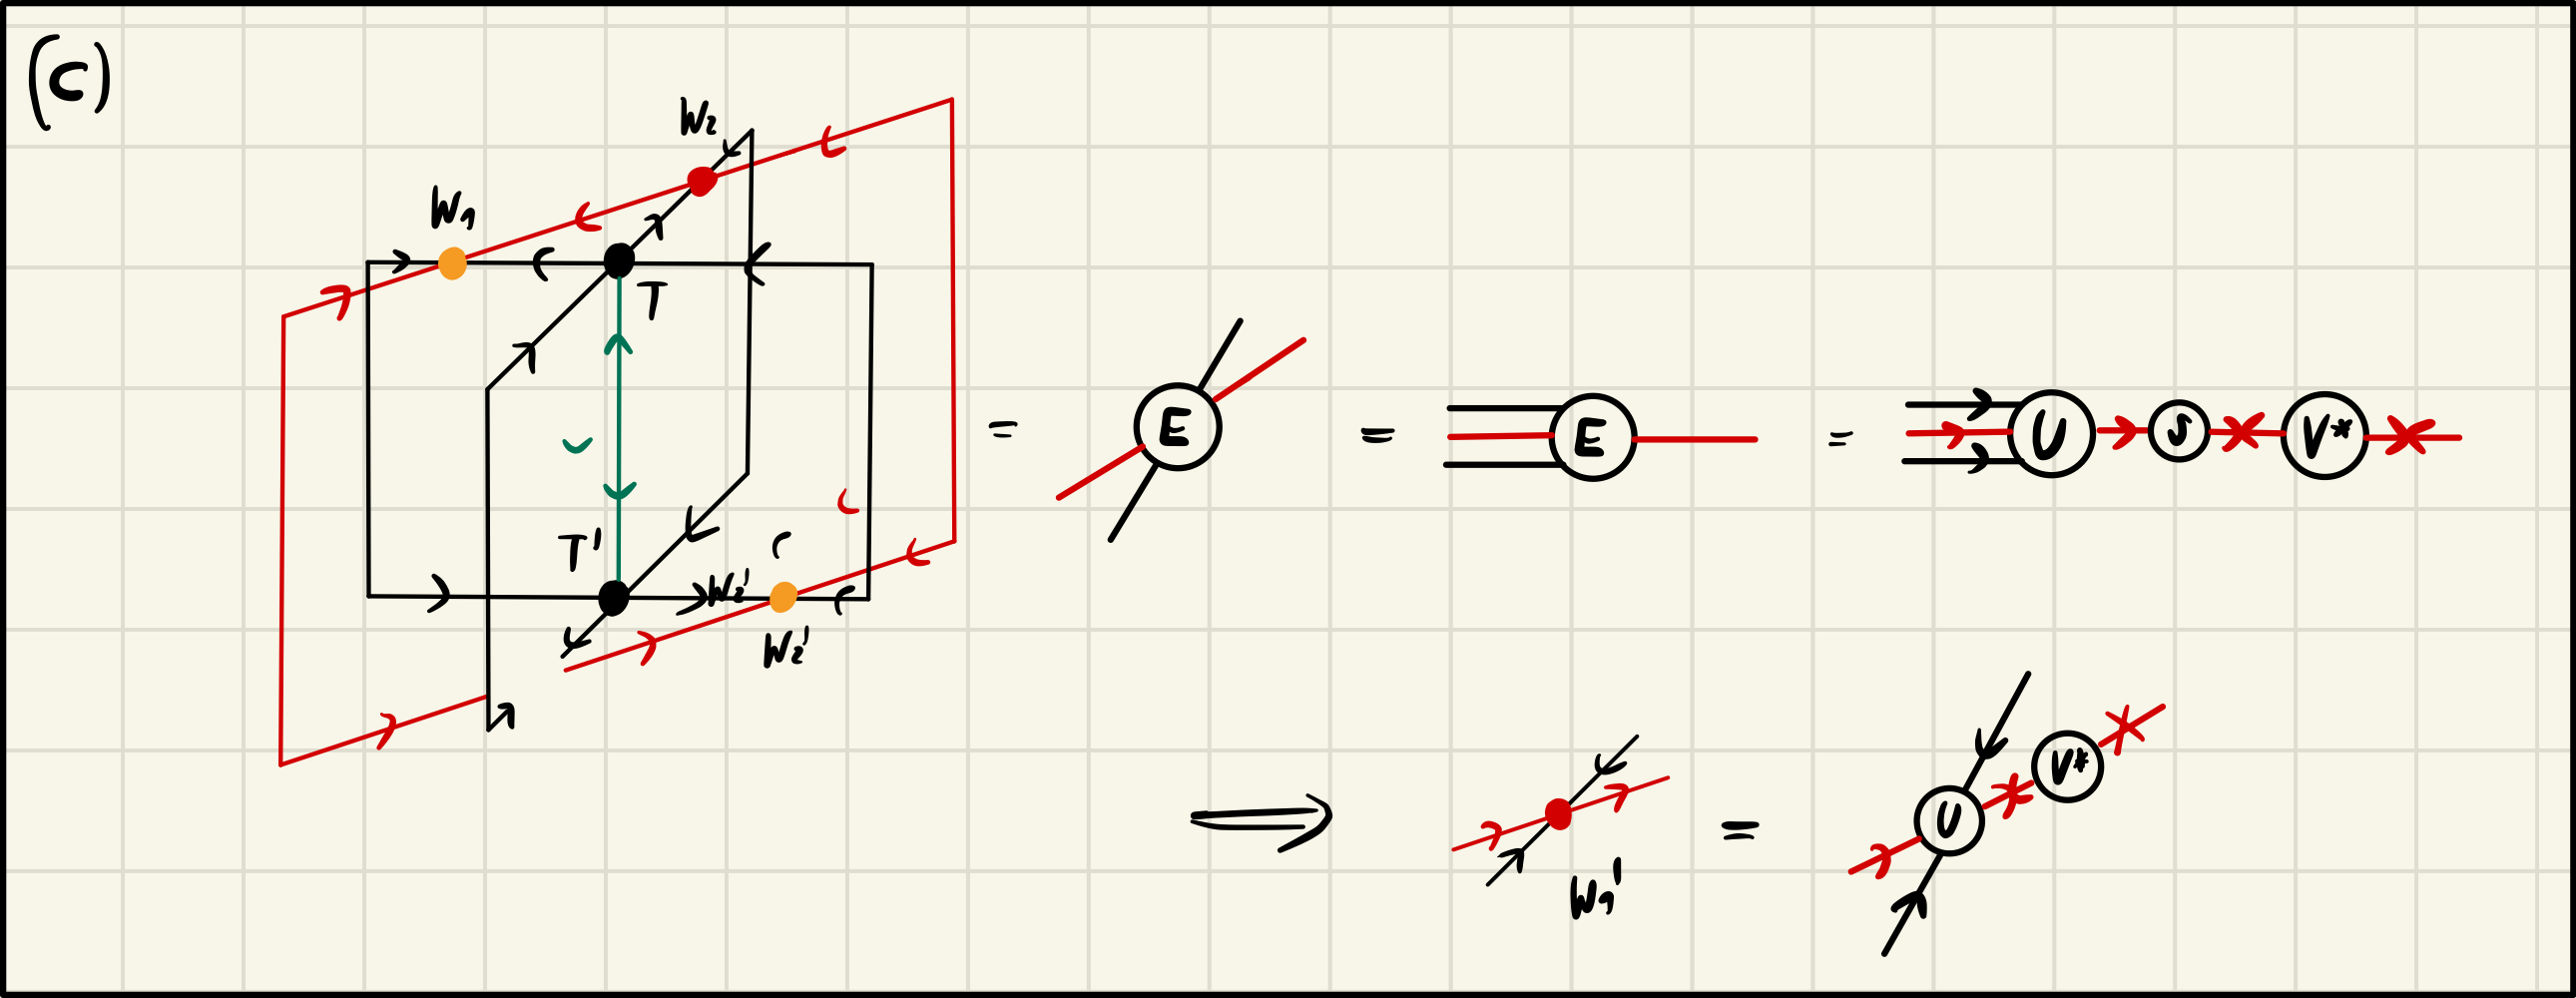
\includegraphics[width=0.7\textwidth]{figures/disoTPS/YB_move_iterate_polar_c.jpeg}
	}
	\subcaptionbox{\label{fig:YB_move_iterate_polar_optimize_T}}
	{%
		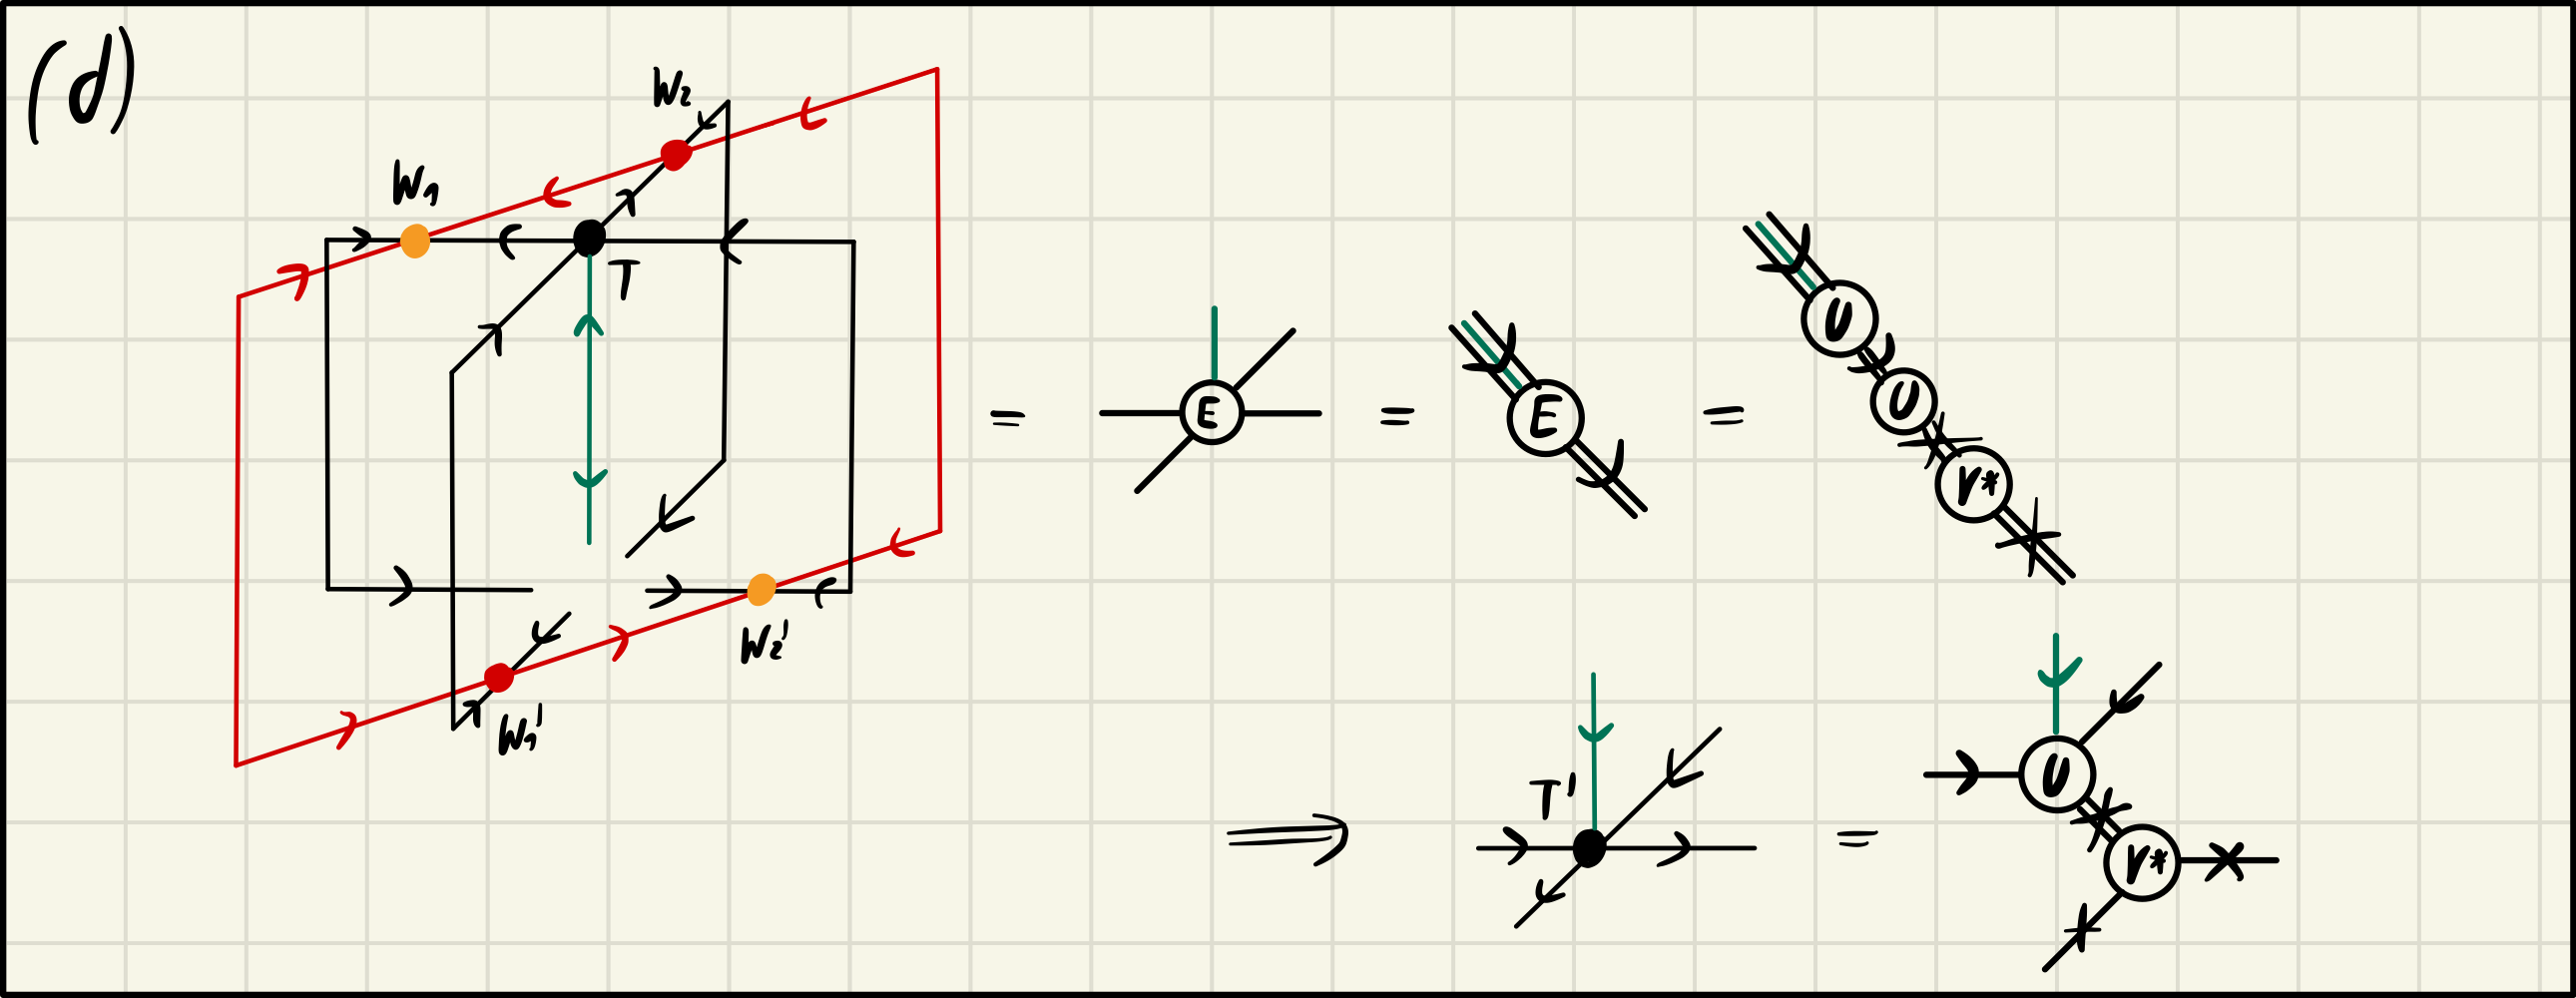
\includegraphics[width=0.7\textwidth]{figures/disoTPS/YB_move_iterate_polar_d.jpeg}
	}
	\caption{\todo{Caption text!}}
	\label{fig:YB_move_iterate_polar}
\end{figure}
